\documentclass[11pt,a4paper]{article}
\usepackage[margin=0.82in]{geometry}
\usepackage[T1]{fontenc}
\usepackage[utf8]{inputenc}
\usepackage{newtxtext,newtxmath}
\usepackage{microtype}
\usepackage{setspace}
\usepackage{parskip}
\usepackage{enumitem}
\usepackage{booktabs}
\usepackage{tabularx}
\usepackage{array}
\usepackage{ragged2e}
\usepackage{titlesec}
\usepackage{tikz}
\usetikzlibrary{arrows.meta,positioning,fit,calc}
\usepackage[hidelinks]{hyperref}
\usepackage{xurl}
\usepackage{fancyhdr}
\usepackage{lastpage}
\usepackage{caption}
\usepackage{float}
\usepackage{multicol}

\setstretch{1.04}
\setlength{\parindent}{1.2em}
\setlength{\parskip}{0.35em}
\setlist[itemize]{leftmargin=1.5em,itemsep=0.15em,topsep=0.2em}
\setlist[enumerate]{leftmargin=1.6em,itemsep=0.15em,topsep=0.2em}
\titleformat{\section}{\large\bfseries\scshape}{\thesection}{0.65em}{}
\titleformat{\subsection}{\normalsize\bfseries}{\thesubsection}{0.55em}{}
\titlespacing*{\section}{0pt}{1.0em}{0.4em}
\titlespacing*{\subsection}{0pt}{0.7em}{0.25em}
\captionsetup{font=small,labelfont=bf}
\pagestyle{fancy}
\fancyhf{}
\lhead{Undergraduate Thesis Proposal}
\rhead{Game-State Fusion for Football BAA}
\cfoot{\thepage\ of \pageref{LastPage}}
\renewcommand{\headrulewidth}{0.3pt}
\setlength{\headheight}{14pt}

\newcommand{\placeholder}[1]{\textit{[#1]}}
\newcommand{\sourceurl}[1]{\url{#1}}
\newcommand{\sourcelink}[2]{\href{#1}{\texttt{#2}}}

\begin{document}

\begin{center}
{\Large\bfseries Evaluating Game-State Fusion for Short-Horizon\\[2pt] Ball Action Anticipation in Football}\par
\vspace{0.45em}
{\large Undergraduate Thesis Proposal}\par
\vspace{1.0em}
\begin{tabular}{rl}
Students: & \placeholder{Names and Student IDs}\\
Department: & \placeholder{Department / University}\\
Supervisor: & \placeholder{Supervisor Name}\\
Date: & 14 August 2026
\end{tabular}
\end{center}
\vspace{0.35em}
\hrule
\vspace{0.6em}

\begin{abstract}
The present inquiry concerns a simple but consequential question: whether an explicit description of the state of a football match can improve the anticipation of actions that have not yet occurred. Ball Action Anticipation (BAA) has recently been formalised in SoccerNet, where a model observes past video and predicts the class and time of ball-related actions in an unseen future interval \cite{dalal2025faantra,cioppa2026}. Existing BAA systems are chiefly visual, while separate work has shown that player positions, velocities, team relations, and longer game context can assist action detection when the action itself is already observable \cite{ochin2025gs,ochin2025beyond}. This proposal therefore studies whether synchronized player game state contributes predictive information in the harder anticipation setting. SoccerTrack v2 is selected because it publicly provides full-pitch panoramic video, Game State Reconstruction (GSR), and Ball Action Spotting (BAS) annotations for ten complete matches \cite{scott2025}. The proposed study compares visual-only, game-state-only, simple-fusion, and relation-aware models under a common evaluation protocol, with particular care given to data alignment, release quality, computational economy, and reproducibility.
\end{abstract}

\section{Problem and Motivation}

Football actions are not determined by appearance alone. A pass, cross, shot, or tackle is also conditioned by the arrangement and motion of the players who make the action possible. Nevertheless, the recently established BAA task asks a model to predict future actions from observations made before those actions become visible. FAANTRA introduced this setting for football and defined each anticipated event by an action class and a timestamp within a future window \cite{dalal2025faantra}. The 2026 SoccerNet challenge fixes the principal task at a 30-second observation period followed by a five-second anticipation period over ten action classes \cite{cioppa2026}.

The difficulty is therefore not merely recognition. The decisive frame is withheld. The model must infer what is likely to happen from the state that precedes it. This makes the structured configuration of the match a natural source of evidence. The proposed thesis asks whether such evidence is genuinely useful, and whether its value extends beyond what can already be inferred from video.

\section{Prior Work and Research Gap}

The proposal rests upon four pieces of established evidence.

\begin{table}[H]
\centering
\small
\begin{tabularx}{\textwidth}{>{\RaggedRight\arraybackslash}p{2.55cm} X X}
\toprule
\textbf{Work} & \textbf{What it establishes} & \textbf{What remains open for this thesis}\\
\midrule
FAANTRA \cite{dalal2025faantra} & Football BAA predicts all future ball actions and their temporal positions from past video. & It does not establish the value of explicit synchronized player game state for anticipation.\\
SoccerNet 2026 \cite{cioppa2026} & The official BAA task uses 30 seconds of observed video and predicts actions in the following five seconds. The reviewed systems remain centered on visual representations, temporal modeling, or VLM-derived semantic context. & The five reviewed technical reports do not document metric per-player GSR trajectories or explicit player-interaction graphs as BAA inputs.\\
Ochin et al. \cite{ochin2025gs} & Player positions, velocities, team information, graph reasoning, and visual features can improve football action detection. & The target action is observable. The study does not test prediction into an unseen future interval.\\
Beyond Pixels \cite{ochin2025beyond} & Longer game-state context and inter-player structure can improve denoising of detected football events. & The task remains detection and sequence correction, not BAA.\\
\bottomrule
\end{tabularx}
\caption{The research gap is a task and information gap, not a claim that graph models or video-state fusion are themselves new.}
\end{table}

The defensible research gap is therefore narrow. Existing football BAA work establishes prediction from past visual evidence. Existing detection work establishes that explicit player game state can be useful when the action is already present. The reviewed literature does not establish whether synchronized metric game state provides complementary value for temporally localized ball actions that occur only in an unobserved future interval. This thesis will test that proposition directly.

The study will not claim to be the first football model to combine video and game state, the first to use player graphs, or the first to predict future football events. Such claims would conflict with established prior work \cite{ochin2025gs,ochin2025beyond}.

\section{Research Questions and Objectives}

\textbf{RQ1.} Does explicit player-level game-state information improve short-horizon Ball Action Anticipation compared with a visual-only model?

\textbf{RQ2.} If game state is useful, does relation-aware modeling of player interactions offer additional value beyond a flat representation of the same information?

The corresponding objectives are:

\begin{enumerate}[label=\arabic*.]
\item derive a reproducible BAA protocol from synchronized SoccerTrack v2 video, GSR, and BAS annotations;
\item construct fair visual-only, game-state-only, and multimodal baselines under a common prediction head;
\item compare simple state fusion with relation-aware player interaction modeling while controlling the underlying input information;
\item evaluate temporal localization, per-class behavior, fold-to-fold variation, and computational cost;
\item demonstrate a small end-to-end inference system without requiring recurring paid infrastructure.
\end{enumerate}

\section{Dataset and Derived Benchmark}

\subsection{SoccerTrack v2}

SoccerTrack v2 contains ten full-length university-level matches, approximately 900 minutes of panoramic 4K video, per-frame GSR annotations, and BAS labels for twelve ball-action classes \cite{scott2025}. The GSR records include metric pitch positions together with tracking and player attributes. The current project documentation states that GSR is aligned to the source panoramic video at 25 frames per second \cite{soccertrackGSR}. These properties make the dataset unusually well suited to a controlled study of visual and structured state information.

\begin{table}[H]
\centering
\small
\begin{tabularx}{\textwidth}{>{\bfseries}p{3.0cm} X}
\toprule
Dataset paper & \sourcelink{https://arxiv.org/abs/2508.01802}{arxiv.org/abs/2508.01802}\\
Canonical dataset & \sourcelink{https://huggingface.co/datasets/atomscott/soccertrack-v2}{huggingface.co/datasets/atomscott/soccertrack-v2}\\
Project page & \sourcelink{https://atomscott.github.io/SoccerTrack-v2/}{atomscott.github.io/SoccerTrack-v2/}\\
Code and loaders & \sourcelink{https://github.com/AtomScott/SoccerTrack-v2}{github.com/AtomScott/SoccerTrack-v2}\\
Google Drive mirror & \sourcelink{https://drive.google.com/drive/folders/1N2Qx2qkFgRtpbHitl2Vh6sLVYGgqkWwn}{Official Drive mirror folder}\\
\bottomrule
\end{tabularx}
\caption{Dataset access. The project presently identifies Hugging Face as the canonical distribution and warns that mirrors may lag \cite{soccertrackLanding}.}
\end{table}

\subsection{Benchmark protocol}

Each evaluation sample will provide up to 30 seconds of historical context and require prediction of all BAS actions in the following five seconds, following the contemporary SoccerNet BAA formulation \cite{cioppa2026}. The model may initially consume a shorter effective context for computational economy, but the future horizon remains fixed at five seconds.

For methodological comparability, the primary label space will use the ten SN-BAA classes, excluding Goal and Free Kick. FAANTRA made this exclusion because those classes were too rare in its test split for stable AP estimates \cite{dalal2025faantra}. Because SoccerTrack v2 has a different class distribution, the complete twelve-class result will also be reported as a secondary analysis rather than silently discarding difficult classes.

The principal evaluation will use match-level grouped cross-validation. No temporal window from a held-out match will appear in training. The final number and identity of folds will be fixed only after the canonical revision has passed the data-quality audit. Performance will be reported using the BAA measures mAP@$\delta$ for $\delta\in\{1,2,3,4,5,\infty\}$ and their average, together with per-class AP and fold variation \cite{dalal2025faantra,cioppa2026}. For finite $\delta$, FAANTRA counts a temporal prediction as correct when it lies within $\delta/2$ seconds of the ground-truth time \cite{dalal2025faantra}.

\subsection{Data integrity}

The current SoccerTrack repository itself records two matters that require caution. First, the shipped GSR files differ structurally from the simplified schema in the documentation, and the maintainers advise consumers to use the actual released structure and supported loaders \cite{soccertrackGSR}. Second, a documented calibration error affects match 132831, whose GSR labels were generated from faulty calibration data and are stated to require regeneration in the shared copy \cite{soccertrackCorrection}. Accordingly, the study will pin a canonical dataset revision, validate BAS-to-GSR-to-video alignment, and exclude or quarantine any match whose corrected state cannot be verified before training.

\section{Method and System Architecture}

The system is deliberately arranged so that the large raw files are handled once, while ordinary model training uses only compact derived representations. This separates data engineering from repeated learning and keeps the experiment within modest computational means.

\begin{figure}[h]
\centering
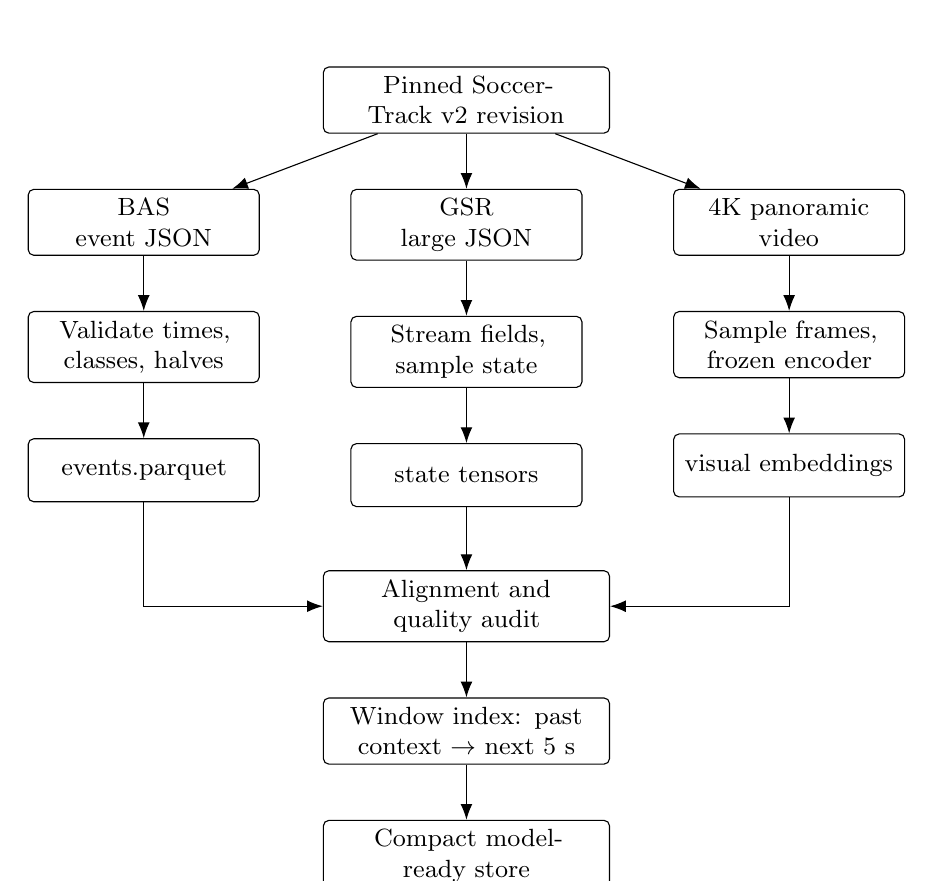
\begin{tikzpicture}[
node distance=7mm and 8mm,
box/.style={draw, rounded corners=2pt, align=center, minimum height=8mm, text width=27mm, font=\small},
wide/.style={draw, rounded corners=2pt, align=center, minimum height=8mm, text width=34mm, font=\small},
arr/.style={-{Latex[length=2mm]}, thin}
]
\node[wide] (source) {Pinned SoccerTrack v2 revision};
\node[box, below left=of source] (bas) {BAS\\event JSON};
\node[box, below=of source] (gsr) {GSR\\large JSON};
\node[box, below right=of source] (vid) {4K panoramic\\video};
\node[box, below=of bas] (be) {Validate times,\\classes, halves};
\node[box, below=of gsr] (ge) {Stream fields,\\sample state};
\node[box, below=of vid] (ve) {Sample frames,\\frozen encoder};
\node[box, below=of be] (bp) {events.parquet};
\node[box, below=of ge] (gp) {state tensors};
\node[box, below=of ve] (vp) {visual embeddings};
\node[wide, below=8mm of gp] (align) {Alignment and quality audit};
\node[wide, below=of align] (win) {Window index: past context $\rightarrow$ next 5 s};
\node[wide, below=of win] (train) {Compact model-ready store};
\draw[arr] (source) -- (bas); \draw[arr] (source) -- (gsr); \draw[arr] (source) -- (vid);
\draw[arr] (bas) -- (be); \draw[arr] (gsr) -- (ge); \draw[arr] (vid) -- (ve);
\draw[arr] (be) -- (bp); \draw[arr] (ge) -- (gp); \draw[arr] (ve) -- (vp);
\draw[arr] (bp) |- (align); \draw[arr] (gp) -- (align); \draw[arr] (vp) |- (align);
\draw[arr] (align) -- (win); \draw[arr] (win) -- (train);
\end{tikzpicture}
\caption{Proposed data architecture. Large raw files are consumed once and replaced by compact indexed representations for repeated experiments.}
\end{figure}

The current GSR documentation warns that a shipped half can be about 2.7 GB and that naïve full-file loading may require roughly 20 GB of memory \cite{soccertrackGSR}. The preprocessing stage will therefore stream only required fields, retain pitch position and player attributes, derive velocity, and downsample the 25 fps state sequence to an initial working rate of 5 Hz. The 5 Hz rate is a starting engineering choice, not an assumed optimum.

Video will likewise be sampled once. An initial rate near 6.25 fps will be used to obtain frozen visual embeddings, after which the 4K video is no longer required during ordinary training. Continuous per-match feature arrays will be stored once, while training windows will contain only indexes into those arrays. This avoids duplicating overlapping clips.

The model study will use a common multi-event prediction head so that differences can be attributed to the available information rather than to different decoders. FAANTRA demonstrates a suitable query-based formulation in which each query predicts action presence, class, and temporal position \cite{dalal2025faantra}. The following controlled models are proposed:

\begin{table}[H]
\centering
\small
\begin{tabularx}{\textwidth}{>{\bfseries}p{1.2cm} p{3.2cm} X}
\toprule
B1 & Visual only & Frozen visual features plus a lightweight temporal encoder.\\
B2 & Game state only & Player position, motion, role, and team relation without visual input.\\
B3 & Simple fusion & Visual representation concatenated with a flat pooled game-state representation.\\
B4 & Flat relations & B3 plus explicit relative position, distance, relative velocity, and team relation, but no graph message passing.\\
B5 & Relation-aware fusion & The same relation information as B4, processed by a lightweight player-interaction graph before fusion with visual context.\\
\bottomrule
\end{tabularx}
\caption{Core experiment ladder. B3 versus B1 addresses RQ1. B5 versus B4 addresses RQ2.}
\end{table}

The relation-aware component is not presented as a new invention. Graph-based player context has already been used in football detection \cite{ochin2025gs}. Its purpose here is to provide a controlled instrument for testing whether relational state representation is useful in anticipation.

\section{Evaluation, Feasibility, and Resource Discipline}

The research will proceed through gates rather than committing the entire compute budget at the outset. A pilot will first use approximately ten minutes from one clean match. It must demonstrate that the canonical data can be downloaded, GSR can be streamed, BAS events can be aligned to both state and video, frozen visual features can be extracted, windows can be generated, and a small anticipation model can reduce its loss and emit class-time predictions. The pilot is a feasibility proof, not a scientific result.

Only after this gate passes will one complete fold be used to establish B1 through B5. Full grouped cross-validation will follow only after the pipeline is stable. This order prevents a preprocessing defect or unsuitable model interface from consuming the majority of the accelerator budget.

The intended Colab plan presently provides 100 compute units, while Google explicitly notes that accelerator types, availability, and runtime limits remain dynamic \cite{colabPricing,colabFAQ}. CPU runtimes will therefore be used for JSON streaming, validation, statistics, and window construction. Accelerator time will be reserved for one-time visual feature extraction and lightweight model training. Resource use will be measured during the pilot and extrapolated before the full run. If the projected cost is excessive, sampling rate or backbone size will be reduced before full extraction.

The final analysis will report mean and variation across match folds, per-class AP, and direct paired differences for the comparisons that answer the two research questions. Absolute results will not be presented as SoccerNet leaderboard scores because SoccerTrack v2 is a different dataset and domain.

\section{Expected Contribution, Scope, and Work Plan}

The anticipated contribution is principally empirical rather than architectural. The work will determine whether explicit player game state contributes information that is absent or insufficient in visual BAA, and whether structured player relations add value beyond a flat state representation. A second contribution will be a reproducible procedure for deriving BAA windows from synchronized SoccerTrack v2 modalities. A compact API demonstration will show how the model may be incorporated into a practical software system, but this engineering layer will not be presented as the scholarly novelty.

The scope is intentionally limited. The thesis will not train a detector, tracker, re-identification system, or calibration system from scratch. It will not undertake cross-dataset transfer, large-scale backbone fine-tuning, or an extensive architecture search. These exclusions are necessary if the principal question is to be answered carefully within one month.

\begin{table}[H]
\centering
\small
\begin{tabularx}{\textwidth}{>{\bfseries}p{1.2cm} X}
\toprule
Week 1 & Pin the canonical dataset revision, complete the alignment audit, run the ten-minute feasibility pilot, and freeze the benchmark folds.\\
Week 2 & Extract compact visual/state representations and establish B1, B2, and B3 on one fold.\\
Week 3 & Implement B4 and B5, debug the controlled comparisons, then run the core models across all folds.\\
Week 4 & Complete essential ablations, per-class and efficiency analysis, write the thesis results, and build the lightweight demonstration system.\\
\bottomrule
\end{tabularx}
\caption{Proposed one-month execution schedule.}
\end{table}

A successful thesis does not require the fusion model to win. If explicit game state improves BAA, the study will identify where that improvement arises. If it does not, the result will still answer a well-defined question that prior detection work leaves unresolved. The scientific obligation is therefore not to guarantee a gain, but to conduct a comparison in which the meaning of either outcome is clear.

\section{Conclusion}

The proposed thesis is built upon a modest proposition. Football anticipation should be examined not only through what the camera sees, but also through the state of the game that gives those images meaning. Prior research has separately established visual Ball Action Anticipation and game-state-assisted action detection. SoccerTrack v2 now makes it possible to place these two lines of work in direct experimental relation. By holding the prediction task and decoder constant while varying the information supplied to the model, the study seeks a clear answer to whether explicit player game state assists the prediction of actions before they occur. The design is deliberately conservative in computation, guarded in its novelty claims, and reproducible in its treatment of data.

\clearpage
\begin{multicols}{2}
\begin{thebibliography}{9}
\scriptsize
\setlength{\itemsep}{0.12em}
\setlength{\parskip}{0pt}

\bibitem{dalal2025faantra}
M. Dalal, A. Xarles, A. Cioppa, S. Giancola, M. Van Droogenbroeck, B. Ghanem, A. Clapés, S. Escalera, and T. B. Moeslund,
``Action Anticipation from SoccerNet Football Video Broadcasts,'' \textit{CVPR Workshops (CVSports)}, 2025.\newline
\sourcelink{https://openaccess.thecvf.com/content/CVPR2025W/CVSPORTS/html/Dalal_Action_Anticipation_from_SoccerNet_Football_Video_Broadcasts_CVPRW_2025_paper.html}{CVF Open Access}

\bibitem{cioppa2026}
A. Cioppa et al., ``SoccerNet 2026 Challenges Results,'' arXiv:2607.07320, 2026.\newline
\sourcelink{https://arxiv.org/abs/2607.07320}{arXiv:2607.07320}

\bibitem{ochin2025gs}
J. Ochin, G. Devineau, B. Stanciulescu, and S. Manitsaris,
``Game State and Spatio-Temporal Action Detection in Soccer Using Graph Neural Networks and 3D Convolutional Networks,'' in \textit{Proceedings of ICPRAM}, pp. 636--646, 2025. doi:10.5220/0013161100003905.\newline
\sourcelink{https://www.scitepress.org/Papers/2025/131611/131611.pdf}{SciTePress PDF}

\bibitem{ochin2025beyond}
J. Ochin, R. Chekroun, B. Stanciulescu, and S. Manitsaris,
``Beyond Pixels: Leveraging the Language of Soccer to Improve Spatio-Temporal Action Detection in Broadcast Videos,'' arXiv:2505.09455, 2025.\newline
\sourcelink{https://arxiv.org/abs/2505.09455}{arXiv:2505.09455}

\bibitem{scott2025}
A. Scott, I. Uchida, K. Kuroda, Y. Kim, and K. Fujii,
``SoccerTrack v2: A Full-Pitch Multi-View Soccer Dataset for Game State Reconstruction,'' arXiv:2508.01802, 2025.\newline
\sourcelink{https://arxiv.org/abs/2508.01802}{arXiv:2508.01802}

\bibitem{soccertrackLanding}
SoccerTrack v2 project documentation, ``SoccerTrack v2 - Full-Pitch Soccer Dataset,'' accessed 14 Aug. 2026.\newline
\sourcelink{https://atomscott.github.io/SoccerTrack-v2/}{Project documentation}

\bibitem{soccertrackGSR}
SoccerTrack v2 repository, ``GSR annotation format,'' current repository documentation, verified 11 Aug. 2026.\newline
\sourcelink{https://github.com/AtomScott/SoccerTrack-v2/blob/main/docs/format-gsr.md}{GSR format documentation}

\bibitem{soccertrackCorrection}
SoccerTrack v2 repository, ``Data corrections: 132831 keypoints,'' current repository documentation, accessed 14 Aug. 2026.\newline
\sourcelink{https://github.com/AtomScott/SoccerTrack-v2/tree/main/data_corrections}{Data-corrections record}

\bibitem{colabPricing}
Google, ``Colab Paid Services Pricing,'' accessed 14 Aug. 2026.\newline
\sourcelink{https://colab.research.google.com/signup}{Colab pricing}

\bibitem{colabFAQ}
Google, ``Google Colab Frequently Asked Questions,'' accessed 14 Aug. 2026.\newline
\sourcelink{https://research.google.com/colaboratory/faq.html}{Colab FAQ}

\end{thebibliography}
\end{multicols}

\end{document}
